\documentclass[11pt,a4paper]{article}

% For an IEEE submission, swap the two lines above for
%   \documentclass[conference]{IEEEtran}
% and delete the geometry package below.
\usepackage[margin=1in]{geometry}
\usepackage[T1]{fontenc}
\usepackage[utf8]{inputenc}
\usepackage{amsmath,amssymb}
\usepackage{booktabs}
\usepackage{graphicx}
\usepackage{subcaption}
\usepackage{xcolor}
\usepackage[numbers,sort&compress]{natbib}
\usepackage[hidelinks]{hyperref}

\graphicspath{{figures/}}

\newcommand{\caveat}[1]{\textcolor{red!70!black}{#1}}

\title{Leakage-Controlled Wafer-Map Defect Pattern Recognition as a Proxy
Pipeline for Silicon-Carbide Power-Device Inspection}

\author{Festus Bett\\
\small Sofia University\\
\small \texttt{festusbett12@gmail.com}}

\date{\today}

\begin{document}
\maketitle

\begin{abstract}
Silicon-carbide (SiC) power devices fail through crystallographic and
process-induced defects that are expensive to find and, once missed, expensive
to ship. Machine-learned inspection is an attractive response, but there is no
large public SiC defect corpus to develop it on. We therefore build and release
a \emph{proxy} pipeline: the methodology, evaluation protocol and deployment
tooling are developed against two public industrial-inspection datasets ---
WM-811K electrical-test wafer maps for supervised pattern recognition, and
MVTec~AD for unsupervised anomaly detection --- so that only the imaging
front-end, not the method, has to be replaced when SiC data becomes available.

The contribution is threefold. First, an evaluation protocol that controls the
leakage specific to this domain: wafers are grouped by lot before splitting,
because wafers from one lot share process history and a random split leaks that
history across the train/test boundary; the split is asserted lot-disjoint at
load time rather than assumed. Second, an explicit treatment of the class
imbalance that dominates wafer-map data --- roughly 85\% of labelled WM-811K
wafers carry no defect pattern, so accuracy is uninformative and macro-F1,
balanced accuracy and defect recall are reported instead --- with four
imbalance strategies exposed as a controlled ablation. Third, a deployment
artifact: a self-describing model bundle that carries the network as ONNX and
TorchScript together with the exact preprocessing contract it was trained
under, verified at export time against the source model, and scoreable on new
wafer maps with nothing but NumPy and an ONNX runtime.

\caveat{The quantitative results reported here come from a synthetic dataset
used to validate that the pipeline executes end to end. The synthetic patterns
are far cleaner than real wafer maps and the near-perfect scores they produce
say nothing about real-world performance.} Section~\ref{sec:protocol-real}
gives the exact protocol and commands for the real WM-811K runs, which require
GPU time and the Kaggle distribution of the dataset.
\end{abstract}

\section{Introduction}

Silicon carbide has displaced silicon in high-voltage power conversion because
its wider bandgap and higher thermal conductivity permit smaller, faster,
hotter-running devices~\citep{kimoto2014sic,kimoto2015material}. The penalty is
material quality. SiC epitaxy carries defect populations that silicon largely
does not --- basal-plane dislocations, micropipes, threading screw
dislocations, triangular ``carrot'' defects --- and a subset of these are
\emph{killer} defects that destroy the blocking capability of any device built
on top of them~\citep{kimoto2015material}. Because a power device occupies a
large die area, a single killer defect removes a disproportionate share of the
wafer's value, and because the devices are safety-critical, an escape is far
more costly than an unnecessary inspection.

This makes defect inspection an obvious target for machine learning and an
awkward one. The obstacle is data: there is no public SiC inspection corpus
comparable in size to the datasets that drove progress in general computer
vision, and the proprietary ones live inside fabs. Work that waits for such a
corpus does not start.

Our response is to treat the problem as two separable halves. The
\emph{imaging front-end} --- what a photoluminescence, optical or X-ray
topography image of a SiC wafer looks like --- is genuinely SiC-specific and
cannot be substituted. The \emph{inspection method} --- how to split
industrial data without leaking, how to train against extreme class imbalance,
which metrics to believe, how to ship a model that a fab engineer can actually
run --- is not. All of it can be developed, tested and stress-tested on public
industrial data, and most of the engineering mistakes available in this problem
can be made and corrected there at no cost.

We therefore develop against two public datasets:

\begin{itemize}
  \item \textbf{WM-811K}~\citep{wu2015wafer}: approximately 811k wafer maps
    from real production, of which about 173k carry one of nine
    human-assigned labels (eight spatial defect patterns plus \texttt{none}).
    A wafer map records the pass/fail outcome of electrical probing per die,
    so the ``image'' is a low-resolution spatial failure signature rather than
    a photograph. The supervised, multi-class track.
  \item \textbf{MVTec~AD}~\citep{bergmann2019mvtec}: high-resolution images of
    industrial objects and textures with pixel-level anomaly masks, trained
    without defective examples. The unsupervised track, which matters because
    a real fab cannot enumerate its defect classes in advance and needs a
    detector that can say ``this is unlike anything normal''.
\end{itemize}

\paragraph{Contributions.}
\begin{enumerate}
  \item A lot-grouped evaluation protocol for wafer-map data, enforced in code
    at every load (\S\ref{sec:splitting}), and the argument for why the
    obvious random split is wrong here.
  \item An imbalance-aware training and reporting setup
    (\S\ref{sec:imbalance}, \S\ref{sec:metrics}), with four strategies
    structured as an ablation rather than a single tuned choice.
  \item A portable, self-verifying deployment artifact
    (\S\ref{sec:deployment}) that separates a trained model from the code that
    trained it, so that applying it to new data requires neither this
    repository nor PyTorch.
  \item A reproducible software pipeline with a synthetic-data path that
    validates every stage before any download (\S\ref{sec:synthetic}), and a
    results harness that regenerates every table in this paper from run
    outputs (\S\ref{sec:repro}).
\end{enumerate}

\section{Related work}

\paragraph{Wafer-map pattern recognition.}
\citet{wu2015wafer} introduced WM-811K along with hand-crafted
rotation-invariant features and similarity ranking, and it has since become the
standard benchmark for the task. \citet{wang2020mixedwm38} extended the problem
to \emph{mixed-type} defects, where several patterns co-occur on one wafer,
releasing MixedWM38 and showing that deformable convolutions help when the
spatial support of a defect is irregular. Our supervised track follows the
single-label WM-811K formulation; the multi-label extension is left as future
work (\S\ref{sec:future}).

\paragraph{Backbones and imbalance.}
We use standard ImageNet backbones --- residual
networks~\citep{he2016resnet} and EfficientNets~\citep{tan2019efficientnet} ---
rather than a bespoke architecture, because the interesting difficulty here is
the data, not the function class. For imbalance we include focal
loss~\citep{lin2017focal} alongside resampling and loss reweighting, and treat
the choice as an empirical question.

\paragraph{Unsupervised industrial anomaly detection.}
MVTec~AD~\citep{bergmann2019mvtec} established the benchmark; PaDiM
\citep{defard2021padim} models patch-embedding distributions, and
PatchCore~\citep{roth2022patchcore} retrieves from a coreset memory bank of
normal patches. Both are attractive for SiC because they require only
defect-free examples for training.

\paragraph{Leakage.}
\citet{kapoor2023leakage} survey how data leakage has produced
irreproducible results across machine-learning-based science, with grouped
data split at the wrong granularity among the recurring causes. Our
lot-grouping discipline is a direct response, and we make it an assertion
rather than a convention.

\section{Data and evaluation protocol}

\subsection{WM-811K}

Each record holds a two-dimensional wafer map whose entries are
$0$ (off-wafer), $1$ (die passed electrical test) and $2$ (die failed),
together with a lot name and, for the labelled subset, one of nine classes:
\texttt{none}, \texttt{Center}, \texttt{Donut}, \texttt{Edge-Loc},
\texttt{Edge-Ring}, \texttt{Loc}, \texttt{Random}, \texttt{Scratch},
\texttt{Near-full}. Unlabelled wafers are dropped. Maps vary in physical size,
so they are resized to a fixed $64\times64$ grid.

Two properties drive every design decision that follows. The classes are
severely imbalanced, with \texttt{none} accounting for roughly 85\% of labelled
wafers. And the records are grouped: many wafers belong to the same lot.

\subsection{Why the split must be grouped by lot}
\label{sec:splitting}

Wafers processed in one lot pass through the same tools, in the same order,
within the same time window. They therefore share process excursions: if a
chamber drifted, every wafer in that lot carries the signature. Splitting
wafers at random places near-duplicate wafers on both sides of the train/test
boundary, and the resulting test score measures partly the model's ability to
recognise \emph{lots it has already seen} rather than defect patterns in
general.

We split by lot with \texttt{GroupShuffleSplit}, holding out 15\% of lots for
validation and 15\% for test. The guarantee is enforced, not documented:
\texttt{assert\_no\_lot\_leakage} recomputes the lot sets of all three splits
and raises if any lot appears in two of them, and it runs both when the split
is created and every time the processed file is loaded. A leak therefore
becomes an immediate, loud failure rather than an inflated number.

Note what this does \emph{not} control. Lot grouping removes within-lot
leakage; it does not make the split chronological, so a model may still be
validated on a time period it was trained across. That limitation is revisited
in \S\ref{sec:threats}.

\subsection{Preprocessing}

Maps are resized with nearest-neighbour interpolation and nothing else. This is
a correctness requirement rather than a preference: bilinear or bicubic
resampling produces intermediate values between $0$, $1$ and $2$, which
correspond to no physical die state and which the model never sees at training
time. Values are then divided by $2$, mapping $\{0,1,2\}$ to
$\{0, 0.5, 1\}$, and the single channel is repeated three times to match the
input geometry ImageNet backbones expect. No ImageNet mean/standard-deviation
normalisation is applied, because the input is a ternary occupancy map rather
than a photograph.

\subsection{Augmentation}

Augmentation is restricted to the dihedral group: the four $90^{\circ}$
rotations and horizontal flips. Wafers are round and have no canonical
orientation, so these transformations map a valid wafer map to another valid
wafer map. Scaling, shearing, perspective warps and colour jitter do not: they
produce maps that could not arise on a real wafer, and several would also break
the $\{0,1,2\}$ value domain. The augmentation is deliberately weak because the
geometry of the data, not a transformation budget, decides what is admissible.

\subsection{Metrics}
\label{sec:metrics}

Accuracy is not reported as a headline number. With \texttt{none} at
approximately 85\% prevalence, a model that predicts \texttt{none}
unconditionally scores about 85\% accuracy while detecting nothing. We report:

\begin{itemize}
  \item \textbf{macro-F1}, the unweighted mean of per-class F1, which gives a
    rare pattern the same weight as the dominant one;
  \item \textbf{balanced accuracy}, the mean per-class recall;
  \item \textbf{defect recall} and \textbf{defect precision}, computed on the
    collapsed binary question ``does this wafer carry any defect pattern?'',
    which is the first question a fab asks and the one with direct cost
    consequences;
  \item \textbf{per-class F1}, because an aggregate can hide a class the model
    has given up on entirely.
\end{itemize}

Model selection uses validation macro-F1. The test split is evaluated once, at
the end, with the best checkpoint.

\subsection{Imbalance strategies}
\label{sec:imbalance}

Four strategies are exposed and compared under an otherwise identical
configuration: (i) \texttt{none}, plain cross-entropy; (ii)
\texttt{weighted\_sampler}, inverse-frequency oversampling of rare classes
within each batch; (iii) \texttt{class\_weights}, inverse-frequency weighted
cross-entropy; and (iv) \texttt{focal}, focal loss~\citep{lin2017focal} with
$\gamma=2$ combined with class weights. Treating this as an ablation rather
than picking one reflects that the right answer depends on the imbalance ratio
and the model, and that the comparison is cheap relative to its informativeness.

\section{Deployment: the model bundle}
\label{sec:deployment}

A training checkpoint is not a deliverable. The checkpoint written by the
training script holds a state dictionary and an architecture name, so
reconstructing a usable model requires this repository, a compatible
torchvision version, and knowledge of the preprocessing contract that lives in
the training code. Handing that to a colleague, or to a fab's inspection
system, does not work.

We therefore define an export step that produces a self-describing
\emph{bundle}:

\begin{itemize}
  \item \texttt{model.onnx} --- the network as a framework-independent
    graph~\citep{onnx}, with weights inlined in the single file rather than
    written to a sidecar, so that nothing can be left behind in transit.
    Scoring it needs only NumPy and an ONNX runtime: no PyTorch, no
    torchvision, none of this repository's code, and not necessarily Python.
  \item \texttt{model.ts} --- a TorchScript copy for callers already running
    PyTorch.
  \item \texttt{bundle.json} --- the class list and index of the
    \texttt{none} class, the input geometry, and the preprocessing contract
    stated explicitly (nearest interpolation, divisor $2.0$, three repeated
    channels, NCHW, no ImageNet normalisation), together with provenance: the
    checkpoint's SHA-256, the recorded test metrics, library versions and the
    export timestamp.
  \item \texttt{model\_card.md} --- what the model is, how it scored, and
    where it should not be trusted.
\end{itemize}

\paragraph{Export-time verification.}
An export that silently diverges from its source model is worse than no export,
so the step verifies rather than asserts. Both the TorchScript and ONNX graphs
are run on a fixed pseudo-random probe batch and compared against the source
PyTorch model; a maximum absolute logit deviation above $10^{-4}$ aborts the
export, and the measured deviations are recorded in the bundle. In our runs
TorchScript reproduces the source model exactly and ONNX agrees to within
$4\times10^{-6}$, with identical \texttt{argmax} decisions.

\paragraph{Inference.}
The companion inference module accepts a bundle directory or zip and scores
whatever form new data arrives in: a single \texttt{.npy} map, a stack,
a processed \texttt{.npz} (optionally filtered to one split), PNG or JPEG
images decoded back through the $\{0,127,255\}$ convention, or a whole
directory. Maps of any size are resized to the bundle's input geometry. Output
is a table with the predicted pattern, its confidence, the collapsed defect
probability $1 - p(\texttt{none})$, and the full per-class distribution.
Predicted patterns can be accompanied by candidate process root causes drawn
from a rule table --- a hypothesis generator for the engineer, explicitly not a
verdict.

Because preprocessing at inference must be the preprocessing the weights were
fitted under, the resize uses OpenCV when it is installed, matching the
training-time call exactly; a NumPy fallback keeps the dependency-free path
available and its one divergence (destination indices whose source coordinate
is an exact integer, where OpenCV's floating-point \texttt{floor} can take the
previous column) is documented rather than hidden. In the normal flow the
question does not arise, because the maps have already been resized once during
preparation and are passed through untouched.

\section{Experiments}

\subsection{Pipeline validation on synthetic data}
\label{sec:synthetic}

Before any download, a generator writes a small dataset with the same schema as
the real distribution --- including unlabelled rows, variable map sizes, lot
structure and a comparable class imbalance --- by drawing the eight defect
patterns as explicit geometric priors (a central disc, an annulus, an edge
ring, an angular edge sector, a local blob, elevated random failure, a linear
scratch, near-total failure) on a circular wafer support with a background
failure rate. The full pipeline then runs on it: preparation, lot-grouped
splitting, CNN training, export and inference.

The purpose is to establish that every stage executes and that the pieces fit
together, which it does: the run reported in Table~\ref{tab:synthetic}
completed, produced a checkpoint, exported cleanly with verified ONNX
agreement, and scored new maps through the inference path.

\caveat{These numbers must not be read as performance.} The synthetic patterns
are generated from the clean geometric templates the model is then asked to
recognise, with no label noise, no ambiguous or overlapping patterns and no
measurement artefacts. Near-perfect scores are the expected outcome of a
correctly wired pipeline on such data, and carry no information about real
wafer maps. They are reported only to document what was actually run.

\subsection{Protocol for the real WM-811K runs}
\label{sec:protocol-real}

The real experiments require the Kaggle distribution of WM-811K
(\texttt{LSWMD.pkl}) and GPU time; the pipeline is configured to run them
unchanged. The intended sequence is: prepare the data once at $64\times64$ with
a lot-grouped split; run the four-way imbalance ablation on a
\texttt{resnet18} backbone; carry the best imbalance strategy to larger
pretrained backbones (\texttt{resnet50}, \texttt{efficientnet\_b3}); and run
YOLO classification baselines on the identical split so the comparison is fair.
Every run logs to MLflow~\citep{mlflow}, selection is on validation macro-F1,
and the test split is touched once per run. Table~\ref{tab:synthetic} is
regenerated from the run outputs by a single script, so completing these runs
fills the table without any manual transcription.

\section{Results}

\begin{table}[t]
\centering
\small
\caption{Test-split results, regenerated by \texttt{paper/make\_results.py}.}
\label{tab:synthetic}
\begin{tabular}{lrrrrr}
\toprule
run & macro-F1 & balanced acc. & accuracy & defect recall & defect precision \\
\midrule
\texttt{resnet18-synthetic} & 0.992 & 0.991 & 0.995 & 1.000 & 1.000 \\
\bottomrule
\end{tabular}
\end{table}


Figure~\ref{fig:curves} shows the training and validation trajectories of the
synthetic run, and Figure~\ref{fig:balance} the class counts per lot-grouped
split. Figure~\ref{fig:samples} shows example maps per class.

\begin{figure}[t]
  \centering
  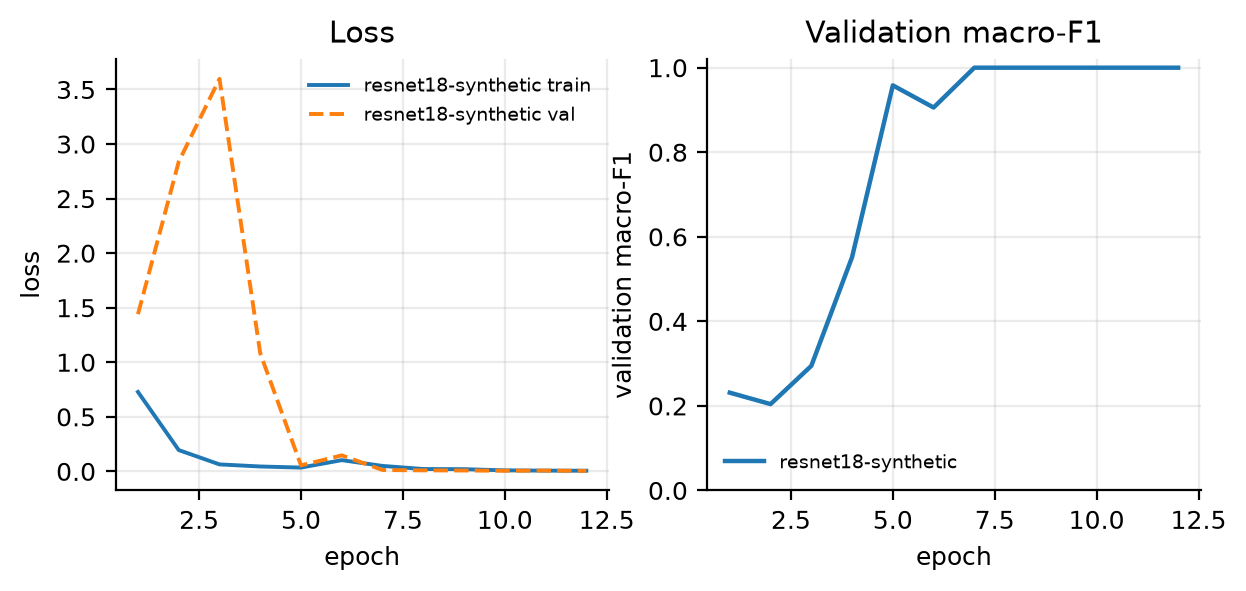
\includegraphics[width=\linewidth]{training_curves.png}
  \caption{Training and validation curves for the synthetic pipeline-validation
  run. The validation macro-F1 saturating near $1.0$ reflects the separability
  of the synthetic patterns, not model quality.}
  \label{fig:curves}
\end{figure}

\begin{figure}[t]
  \centering
  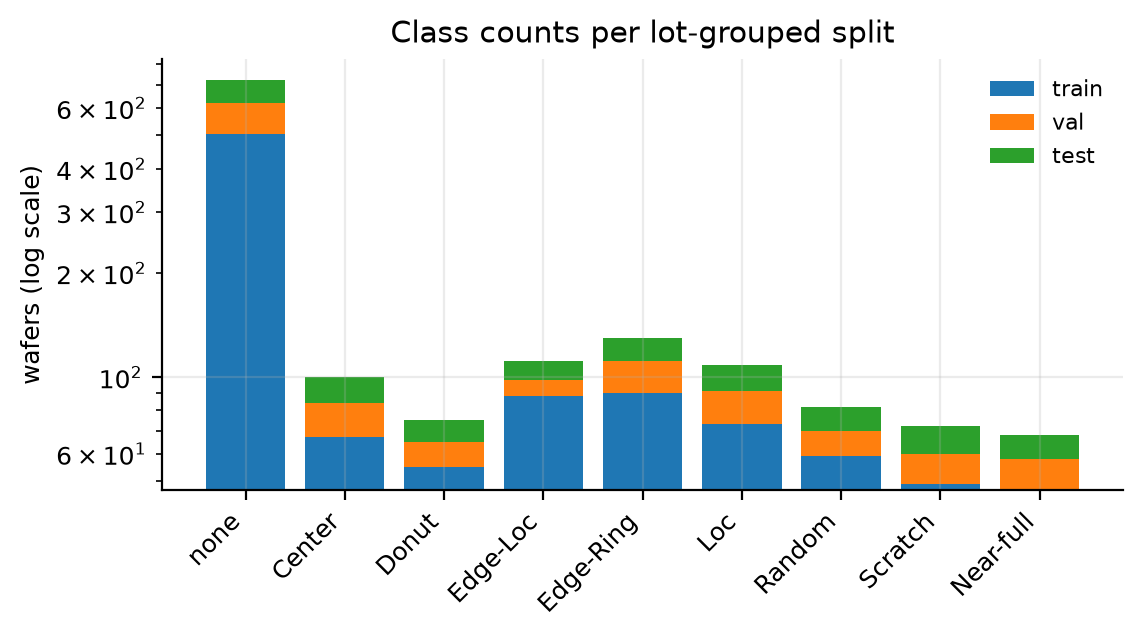
\includegraphics[width=\linewidth]{class_balance.png}
  \caption{Class counts per split (log scale) after lot-grouped splitting. The
  real WM-811K distribution is considerably more skewed, with \texttt{none} at
  roughly 85\%.}
  \label{fig:balance}
\end{figure}

\begin{figure}[t]
  \centering
  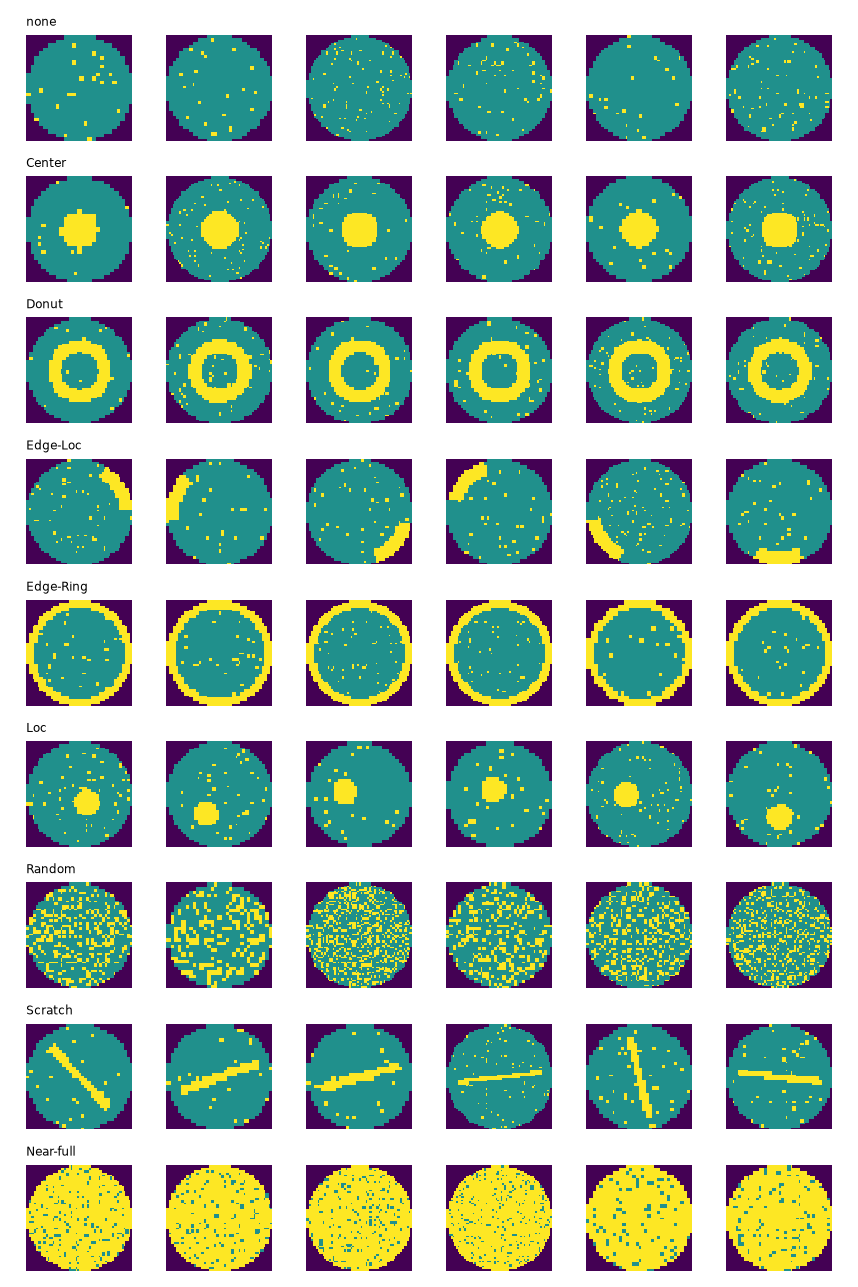
\includegraphics[width=0.78\linewidth]{samples.png}
  \caption{Example wafer maps per class from the prepared dataset.}
  \label{fig:samples}
\end{figure}

\section{Threats to validity}
\label{sec:threats}

\paragraph{The reported numbers are not real-data performance.} This is the
dominant limitation and is restated here deliberately: the quantitative results
come from synthetic data generated to validate the pipeline. No claim about
real WM-811K or SiC performance is supported by them.

\paragraph{Lot grouping is necessary, not sufficient.} Grouping by lot removes
within-lot leakage. It does not make the evaluation chronological, so a model
can still be validated on a time window it was trained across, and slow tool
drift remains uncontrolled. A chronological, lot-disjoint protocol would be
strictly stronger and is the natural next hardening step.

\paragraph{Label noise in WM-811K.} The labels are human-assigned and the
dataset is known to contain ambiguous and contested cases; mixed-type wafers in
particular are forced into a single class by the formulation we adopt. This
bounds achievable macro-F1 by an unknown amount.

\paragraph{The proxy gap is real.} A wafer map is a per-die pass/fail lattice
produced by electrical probing. A SiC inspection image is a photoluminescence,
optical or X-ray topography measurement of crystal structure. They differ in
modality, resolution and defect physics. What transfers from this work is the
protocol, the metric discipline and the deployment machinery; the trained
weights should not be expected to transfer at all, and the model card says so.

\paragraph{Closed-set classification.} The classifier assigns every wafer to
one of nine known classes and cannot abstain. A novel excursion signature will
be forced into the nearest class with possibly high confidence. This is the
specific gap the unsupervised anomaly-detection track exists to fill, and until
that track is run on real data the system has no principled ``something else''
response.

\paragraph{Single seed.} Runs reported here use one seed. Differences between
imbalance strategies should not be interpreted before they are shown to exceed
seed-to-seed variation.

\section{Reproducibility}
\label{sec:repro}

Every stage runs from the command line with pinned seeds, and the dataset
loader re-verifies the lot-disjointness invariant on each load. The synthetic
validation path requires no downloads and runs on CPU in a few minutes.
Experiment metadata, parameters and metrics are logged to
MLflow~\citep{mlflow}; model artifacts are exported with their checkpoint
SHA-256 and library versions recorded in the bundle. The tables and figures in
this paper are produced by \texttt{paper/make\_results.py} directly from the
run outputs, so a stale number in the manuscript is a regenerable artefact
rather than a transcription error. The implementation uses
PyTorch~\citep{paszke2019pytorch} and scikit-learn~\citep{pedregosa2011scikit}.

\section{Conclusion and future work}
\label{sec:future}

We have described a defect-inspection pipeline for SiC power devices built
deliberately on public proxy data, so that the parts of the problem that are
not SiC-specific --- splitting, imbalance, metric choice, and shipping a model
somebody else can run --- can be solved now and the SiC-specific imaging
front-end substituted later. The evaluation protocol enforces lot-disjoint
splits as a runtime invariant; the reporting avoids the accuracy trap that an
85\%-majority dataset sets; and the deployment artifact separates a trained
model from the code that produced it, verified against its source at export
time.

The immediate next step is to complete the real WM-811K runs of
\S\ref{sec:protocol-real} and populate Table~\ref{tab:synthetic} with results
that mean something. Beyond that: a chronological, lot-disjoint split to
control drift as well as grouping; the multi-label mixed-type formulation of
\citet{wang2020mixedwm38}, which is closer to how defects actually co-occur;
the MVTec~AD anomaly-detection track, to give the system an open-set response;
seed repetitions with confidence intervals before any strategy is declared
better; and finally transfer to real SiC photoluminescence or X-ray topography
imagery, where the proxy assumption is finally tested rather than relied upon.

\section*{Data and code availability}

Code, the synthetic generator, the export and inference tooling and this
manuscript are in the project repository. WM-811K is distributed on
Kaggle~\citep{wu2015wafer}; MVTec~AD is available from its
authors~\citep{bergmann2019mvtec}.

\bibliographystyle{plainnat}
\bibliography{refs}

\end{document}
